\begin{figure}[t]
\centering
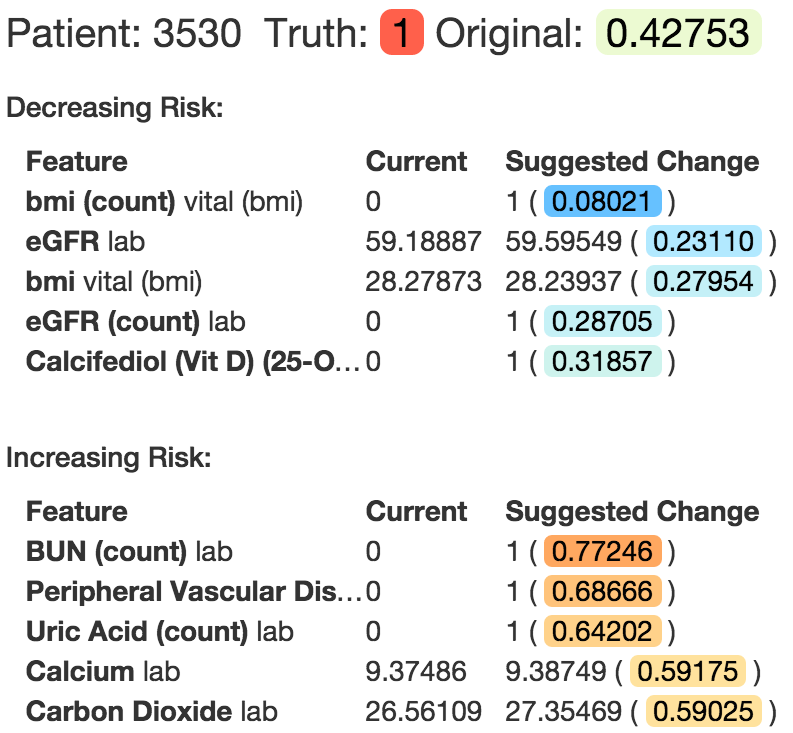
\includegraphics[width=0.5\linewidth]{prospector/patient_summary} % 0.7
\caption[The summary of one patient.]{
The summary of one patient. The header line indicates the patient id, the ground truth, and the predicted
risk.
For both decreasing and increasing the predicted risk the top 5 most impactful features are shown.
Each feature shows its current value and the suggested change with the highest impact along with how the predicted risk would change.
}
\label{figs:summary}
\end{figure}